\documentclass{article}
\usepackage[final]{nips_2017}
\usepackage[utf8]{inputenc} % allow utf-8 input
\usepackage[T1]{fontenc}    % use 8-bit T1 fonts
\usepackage{hyperref}       % hyperlinks
\usepackage{url}            % simple URL typesetting
\usepackage{booktabs}       % professional-quality tables
\usepackage{amsfonts}       % blackboard math symbols
\usepackage{nicefrac}       % compact symbols for 1/2, etc.
\usepackage{microtype}      % microtypography
\usepackage{graphicx}
\usepackage{amsmath}
\usepackage{tikz}
\usetikzlibrary{positioning, shapes.geometric, arrows.meta}
\usepackage{natbib}
\bibliographystyle{unsrtnat}
\usepackage{hyperref}
\usepackage{float}
\usepackage{xcolor}
\usepackage{tcolorbox}
\usepackage{xcolor,soul}
\sethlcolor{cyan!30} % Sets light blue as highlight color

\newcommand{\hlblue}[1]{\hl{#1}}

\title{Automated LaTeX Code Generation from Handwritten Mathematical Expressions \\
Category: Computer Vision}

\author{
  Jayaprakash Sundararaj \\
  \texttt{osjp@stanford.edu}  \\
  \AND
  Akhil Vyas \\
  \texttt{avyas21@stanford.edu}  \\
  \AND
  Benjamin Gonzalez-Maldonado \\
  \texttt{bengm@stanford.edu } \\
}

\begin{document}
% \nipsfinalcopy is no longer used

\begin{center}

\includegraphics[width=3cm, height=0.7cm]{CS230}
\end{center}

\maketitle

\begin{abstract}
Training a model that learns handwritten mathematical expressions from images and generates equivalent LaTeX code. The goal is experiment and study different model architectures (CNN, LSTM, etc) and hyper-parameters, evaluate the with different evaluation metrics, and share our finding.
\end{abstract}

\section{Introduction}	

Converting handwritten mathematical expressions into digital formats is time consuming, specifically LaTeX code. Our goal is to train a ML model that is capable of encoding handwritten notes and converting to the source code seamlessly. The input to our algorithm is an image of a handwritten mathematical expression. The challenge of our project is to convert an image to a text LaTeX sequence which will require the use of both computer vision and NLP techniques. We will use concepts related to these areas that we learn from this course to train the model. We will explore different evaluation metrics (text based, and image based), and share our findings.

% Explain the problem and why it is important. Discuss your motivation for pursuing this
% problem. Give some background if necessary. Clearly state what the input and output
% is. Be very explicit: “The input to our algorithm is an {image, amplitude, patient age,
% rainfall measurements, grayscale video, etc.}. We then use a {SVM, neural network, linear
% regression, etc.} to output a predicted {age, stock price, cancer type, music genre, etc.}.”
% This is very important since different teams have different inputs/outputs spanning different
% application domains. Being explicit about this makes it easier for readers. If you are using
% your project for multiple classes, add a paragraph explaining which components of the
% project were used for each class.


\section{Dataset and Features}

We will use the datasets from two main repositories: \texttt{Im2latex-100k} (\cite{kanervisto_2016_56198}) and \texttt{Im2latex-230k} (\cite{gervais2024mathwritingdatasethandwrittenmathematical}). The \texttt{Im2latex-100k} (\cite{kanervisto_2016_56198}) dataset, available at \href{https://zenodo.org/records/11230382}{Zenodo}, contains 100,000 image-formula pairs. The \texttt{Im2latex-230k} (\cite{gervais2024mathwritingdatasethandwrittenmathematical}) 
 dataset, also known as \texttt{Im2latexv2}, contains 230,000 samples. It includes both OpenAI-generated and handwritten examples, further enhancing the diversity of the data. This dataset is available at \href{https://im2markup.yuntiandeng.com/data/}{Im2markup}. The training data format is \texttt{<image file name> <formula id>}.
 
 The dataset disk size is 849 MB. The images are gray scales with 50x200 pixels. The numbers of symbols (\autoref{fig:formula_length}) in the latex formulas vary from range varies from 1 to 150 symbols. Voabulary contains 540 symbols, refer \autoref{fig:vocab_freq_1} and \autoref{fig:vocab_freq_2} for the list of popular and least occurring symbols with their frequency.
 
\begin{figure}
    \centering
    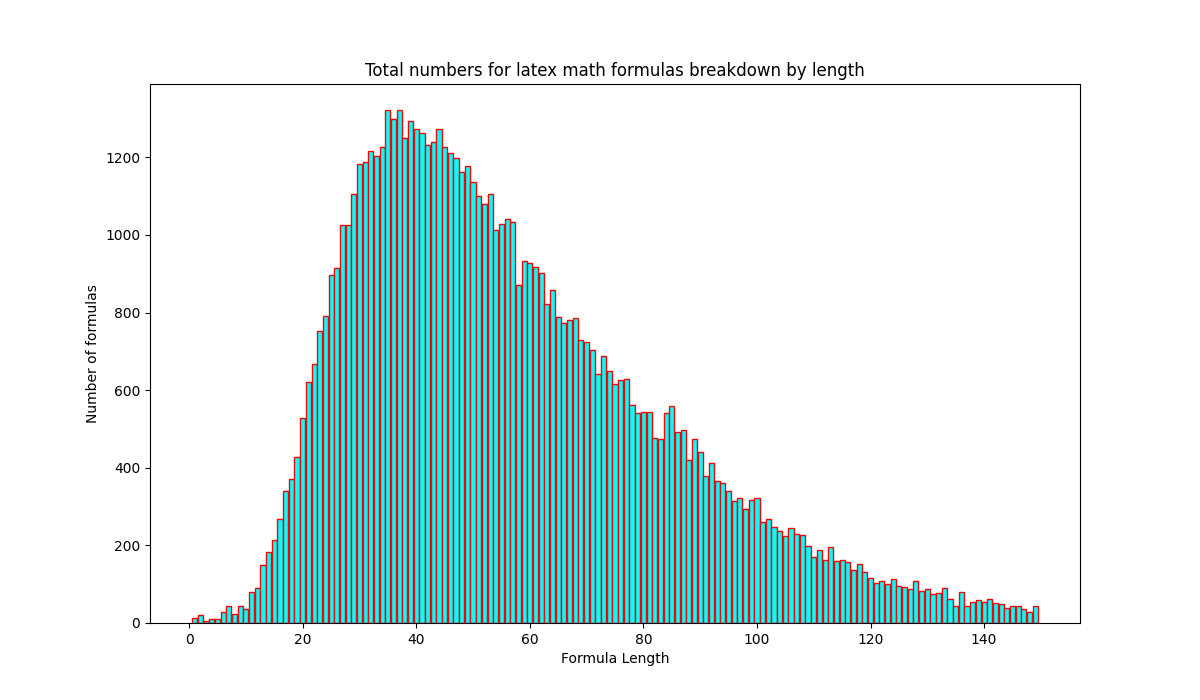
\includegraphics[scale=0.4]{fig_latex_formula_length.png}
    \caption{Formulas breakdown by length}
    \label{fig:formula_length}
\end{figure}


\section{Experiments}

\subsection{Setup}
We use the single AWS P2.xlarge instance (tesla 80 GPU) for training. The training time varies between  1 hr 30 mins and 2 hrs. We use the `sparse categorical loss` with `adam` optimizer for 20 epoches. These hyperparameter are not modified between different configurations to observe the differences in outcome.

\subsection{CNN encoder and GRU/LSTM}
As a baseline, We use the CNN Encoder to encode the image input of resized image (50x200) with 1 channel (greyscale). We use 3x3 convolutional filter followed by 2x2 max pooling layer. This previous block is repeated three times and followed fully connected layer.

\begin{figure}[H]
    \centering
    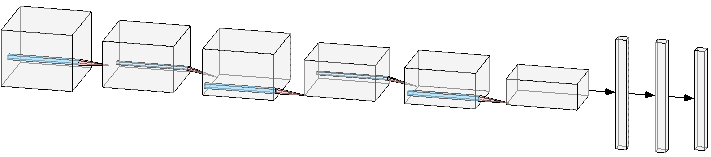
\includegraphics[scale=0.6]{cnn_architecture.png}
    \caption{Encoder architecture consists of 3 convolution-max pooling blocks (50,200) -> (25,100) -> (12,5) which is flattened and fed into Dense layer (256 units)  }	
    \label{fig:cnn_lstm}
\end{figure}

During decoding, We compute the embedding for formula tokens and concatenated with image encoded embedding. The concatenation of image and token embedding fed into LSTM/GRU units, followed by fully connected network. The activation is softmax.  Overall model architecture is: 
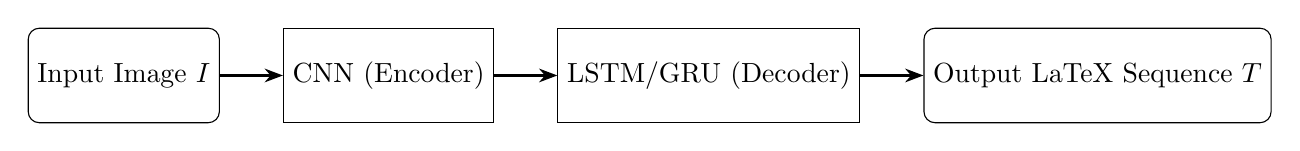
\begin{tikzpicture}[
    node distance=1cm, 
    every node/.style={rectangle, draw, minimum height=1.2cm, minimum width=1cm, align=center},
    arrow/.style={-Stealth, thick}
]

% Nodes
\node (input) [rounded corners] {Input Image \(I\)};
\node (cnn) [right=0.8cm of input] {CNN (Encoder)};
\node (lstm) [right=0.8cm of cnn] {LSTM/GRU (Decoder)};
\node (output) [right=0.8cm of lstm, rounded corners] {Output LaTeX Sequence \(T\)};

% Arrows
\draw [arrow] (input) -- (cnn);
\draw [arrow] (cnn) -- (lstm);
\draw [arrow] (lstm) -- (output);

\end{tikzpicture}

Here are the training curves with  CNN - LSTM/GRU architectures:
\newline \newline
 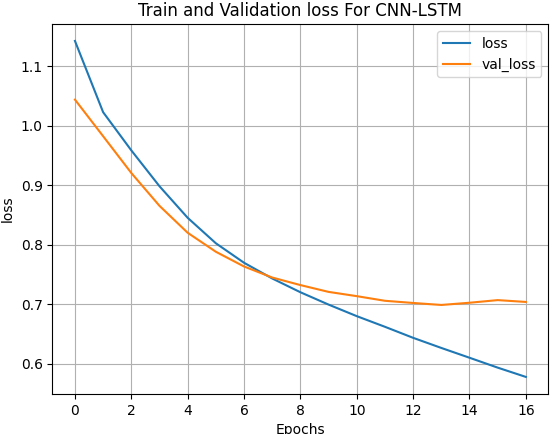
\includegraphics[scale=0.45]{lstm_training.png}
 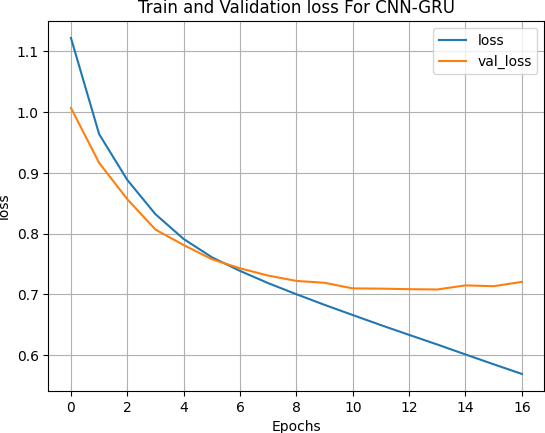
\includegraphics[scale=0.45]{gru_training.png}


\subsection{LSTM with funetuning with pretrained Resnet50}

In this experiment, we use the pretained ResNet50 model as a encoder (98Mb disk size). However, ResNet50 expects the image with fixed size 254x254 and 3 channels. Our input images are grey scale. So, we transform the input image to the ResNet50 input using \verb|tf.keras.layers.Lambda(lambda x: tf.image.grayscale_to_rgb(x)|.

%\begin{figure}[H]
%    \centering
 %   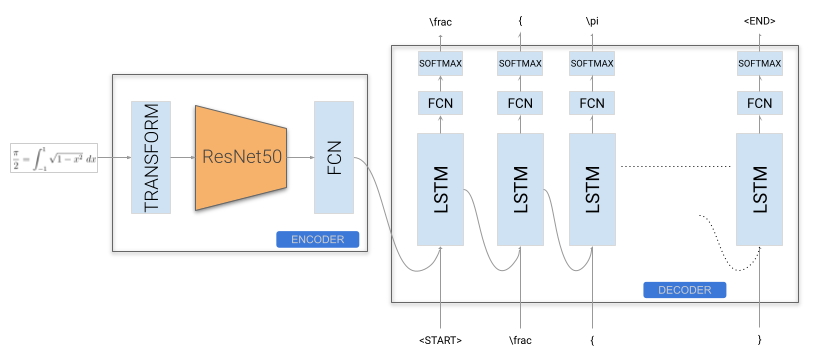
\includegraphics[scale=0.42]{fig_resnet_LSTM.png}
%    \caption{Pretrained ResNet50 Encoder with LSTM Decoder.}
  %  \label{fig:resnet_lstm}
%\end{figure}

\section{Future Work}

\begin{enumerate}
 \item \hlblue{Work in-progress by Ben}  Compute the \textbf{accuracy} between images generated from original latex code and generated latex code. Also look at BLEU score, Levenshtein Distance.
\item  We're aiming to inspect the accuracy losses and ensure that mis-predicted examples are correctly identified with increased weighting. 
\item \hlblue{Work in Progress by Akhil}. We're in the middle of trying to explore VisionTransformer architecture for this task.   \item \hlblue{Work in Progress by JP} During inference time, we're using the greedy algorithm to pick the token with maximum logit score at every time. It terminates when the \verb|<END>| token is predicted or reaches the maximum sequence length. We will explore beam search in this experiment. 
\end{enumerate}


\medskip

\nocite{*}
\bibliography{sample}


\end{document}